\documentclass{beamer}
\usepackage[utf8]{inputenc}
\usepackage{graphicx}
\usepackage{subfig}
\author[Sowmya Vajjala]{Instructor: Sowmya Vajjala}


\title[LING 120]{LING 120, Fall 2017 \\ Language and Computers}

\date{20 September 2017}

\institute{Iowa State University, USA}

%%%%%%%%%%%%%%%%%%%%%%%%%%%

\begin{document}

\begin{frame}\titlepage
\end{frame}

\begin{frame}
\frametitle{Class outline}%5minutes
\begin{enumerate}
\item Review of last class
\item Introduction to searching the web
\item Issues related to language
\end{enumerate}
\end{frame}

\begin{frame}
\frametitle{Different types of data}%5minutes
\begin{enumerate}
\item Structured - Very organized (e.g., a library database - every book has a title, an author, a publisher, other attributes such as number of pages etc.)
\item Unstructured - free-flowing text from which we should extract what we want (e.g., your typical google search)
\item Semi-structured - where the data is generally unstructured, but there are certain patterns we see, which makes it easy to extract content (e.g., if we want to extract all email addresses from a text).
\end{enumerate}
\end{frame}

\begin{frame}
\frametitle{Evaluating Search Results}%5minutes
\begin{enumerate}
\item We know how to evaluate search results based on our information need. How do we decide whether a search system is generally good? \pause
\item Relevance: Whether the result a search showed us is actually relevant for the user's need. \pause
\item Precision: Of all results returned by the search, how many are actually relevant?
\item Recall: Of all the results that are relevant, how many did the search engine manage to retrieve as relevant? 
\item The goal of a good search engine is to provide 100\% precision and 100\% recall. 
\end{enumerate}
\end{frame}

\begin{frame}
\frametitle{Precision and Recall: Competing Priorities}%5minutes
\begin{enumerate}
\item How do we achieve 100\% recall? \pause
\\ $\Rightarrow$ Just show up everything in the world - that will automatically achieve 100\% recall (How??) \pause
\item How do we achieve 100\% precision? \pause
\\ $\Rightarrow$ return that small set of webpages which you are absolutely sure of. (Great, what is the problem then?) \pause
\item Often, the goal is to reach a balance between precision and recall. 
\end{enumerate}
\end{frame}

\begin{frame} %10-15 min
\frametitle{Last class: A question about "searching"}
Work in groups of 2--3 people, think about a solution for this problem, and return your answers to me giving the names of your team members. You can also submit online on Canvas. 
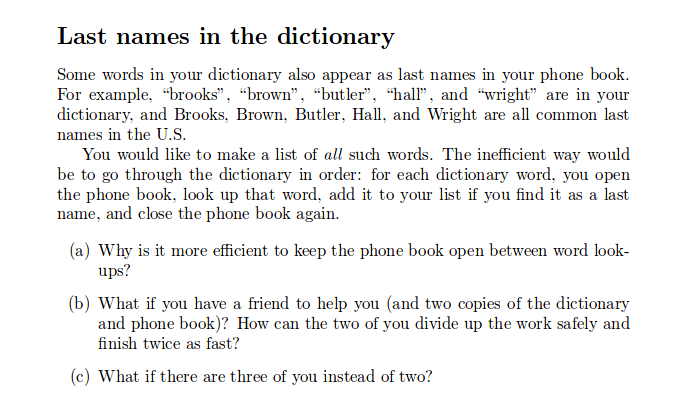
\includegraphics[width=0.9\textwidth]{18Sep-120Exercise.png}
\tiny source: \url{http://nacloweb.org/resources/problems/sample/Phonebook.pdf}
\end{frame}

\begin{frame} %10-15 min
\frametitle{Answer discussion}
\url{http://nacloweb.org/resources/problems/sample/Phonebook-solution.pdf}
\end{frame}

\begin{frame}
\frametitle{}
\begin{center}
\Large Search Engines
\end{center}
\end{frame}

%Linguistic issues in search
\begin{frame}
\frametitle{Typical usage of a search engine}
\begin{itemize}
\item Let us say we want to search for something ("Iowa State University").
\item We go to google and type that string in and choose to search.
\item Google returns you lots of results, ranked in some way and paginated.
\item We evaluate the results (by looking at the top few results) and seeing if they are relevant \pause
\item If we are unhappy, we reformulate the query and search repeat the above process again. \pause
\item From the perspective of google, if we click a result, it can be considered somewhat relevant. 
\end{itemize}
\end{frame}

\begin{frame}
\frametitle{How does a search engine prioritize one page over the other?}
\framesubtitle{Some simple intuitions}
\begin{itemize}
\item If I am searching for something, and there is a webpage with that "something" in the title, or in URL etc, may be that should be ranked first.
\item If there is a Wikipedia page, may be that can show up first.
\item If it is a movie, may be the IMDB page can show up first.
\item If we are searching for a well-known personality's name and that person has a twitter handle, that should also be seen in top results.
\item If there are "advertisements" relevant to my query, they need to be displayed too! (search for, say, "language learning" on google). 
\item Similar results (or many results from same website) should be grouped together.
\end{itemize}
\end{frame}

\begin{frame}
\frametitle{Language related issues in a search engine}
\begin{itemize}
\item Should we consider upper case/lower case differences between words? or should we treat them the same? \pause
\item Should I look for exact spellings or may be approximate ones too? \pause (T\"ubingen, Tuebingen, Tubingen - all can refer to the same German town). \pause 
\item Should I do "stemming", which is basically stripping off word endings? (i.e., car, cars will both be matched). What is the advantage? \pause
\item How can I store all information on the web? How can I just search instantly? \pause
\item Ads again: How can I show ads relevant to search query? (Why is it important?)
\end{itemize}
\end{frame}

\begin{frame}
\frametitle{How does a search engine work?}
\framesubtitle{Which of those require some analysis of language?}
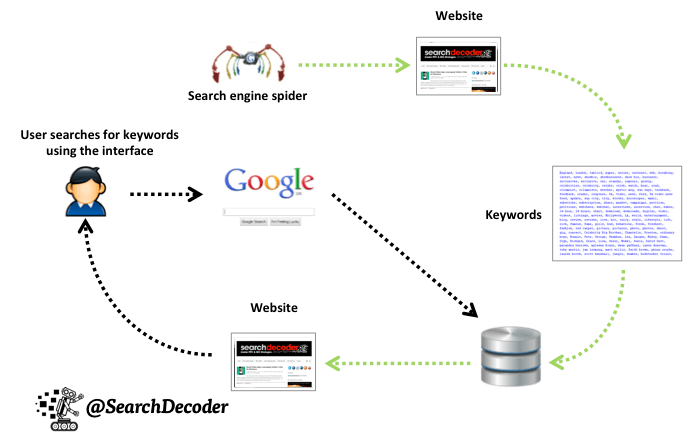
\includegraphics[width=0.9\textwidth]{search.png}
\medskip \tiny source: \url{https://www.searchdecoder.com/how-do-search-engines-work}
\end{frame}

\begin{frame}
\frametitle{Language analysis in search}
\begin{itemize}
\item "Crawling" to "Indexing": How do we get plain text from webpages? (What is the issue?)
\item "Indexing: Purpose is to store all the collected data in an efficient way.
\item Understanding a query (may be also translation if it involve cross-language search)
\item What snippets need to be shown under a search result?
\item Grouping results into categories
\end{itemize}
\end{frame}

\begin{frame}
\frametitle{Indexing}
\begin{itemize}
\item One popular indexing structure is: Term-Document Matrix.
\item All words as rows, webpages in which they appear as columns.
\item Counts or just binary numbers as entries in this matrix. \pause
\item It is often common to remove "stop words" i.e., removing extremely frequent words such as I, the, a, is etc. (Why?) \pause
\item A more efficient way of representing a TDM is something called inverted index, where you just list the document IDs instead of that big matrix. 
\end{itemize}
\end{frame}

\begin{frame}
\frametitle{TDM and Inverted Index}
%2 pictures.
\begin{figure}%
    \centering
    \subfloat[Term Document Matrix]{{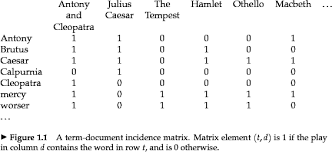
\includegraphics[width=5cm]{tdm.png} }}%
    \qquad \pause
    \subfloat[Inverted Index]{{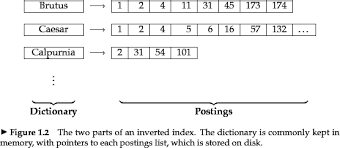
\includegraphics[width=5cm]{invertedindex.png} }}%
   % \caption{2 Figures side by side}%
    \label{fig:example}%
\end{figure}
\pause
\begin{itemize}
\item TDM for WWW is incredibly huge. 
\item Modern search engines use several other characteristics as well (beyond words and phrases).
\end{itemize}
\end{frame}

\begin{frame}
\frametitle{How is this useful when someone searches?}
If I search for "Iowa" AND "state" AND "university" - I look for documents that contain all three words and show these!
\end{frame}

\begin{frame} %10-15 min
\frametitle{Small Question}
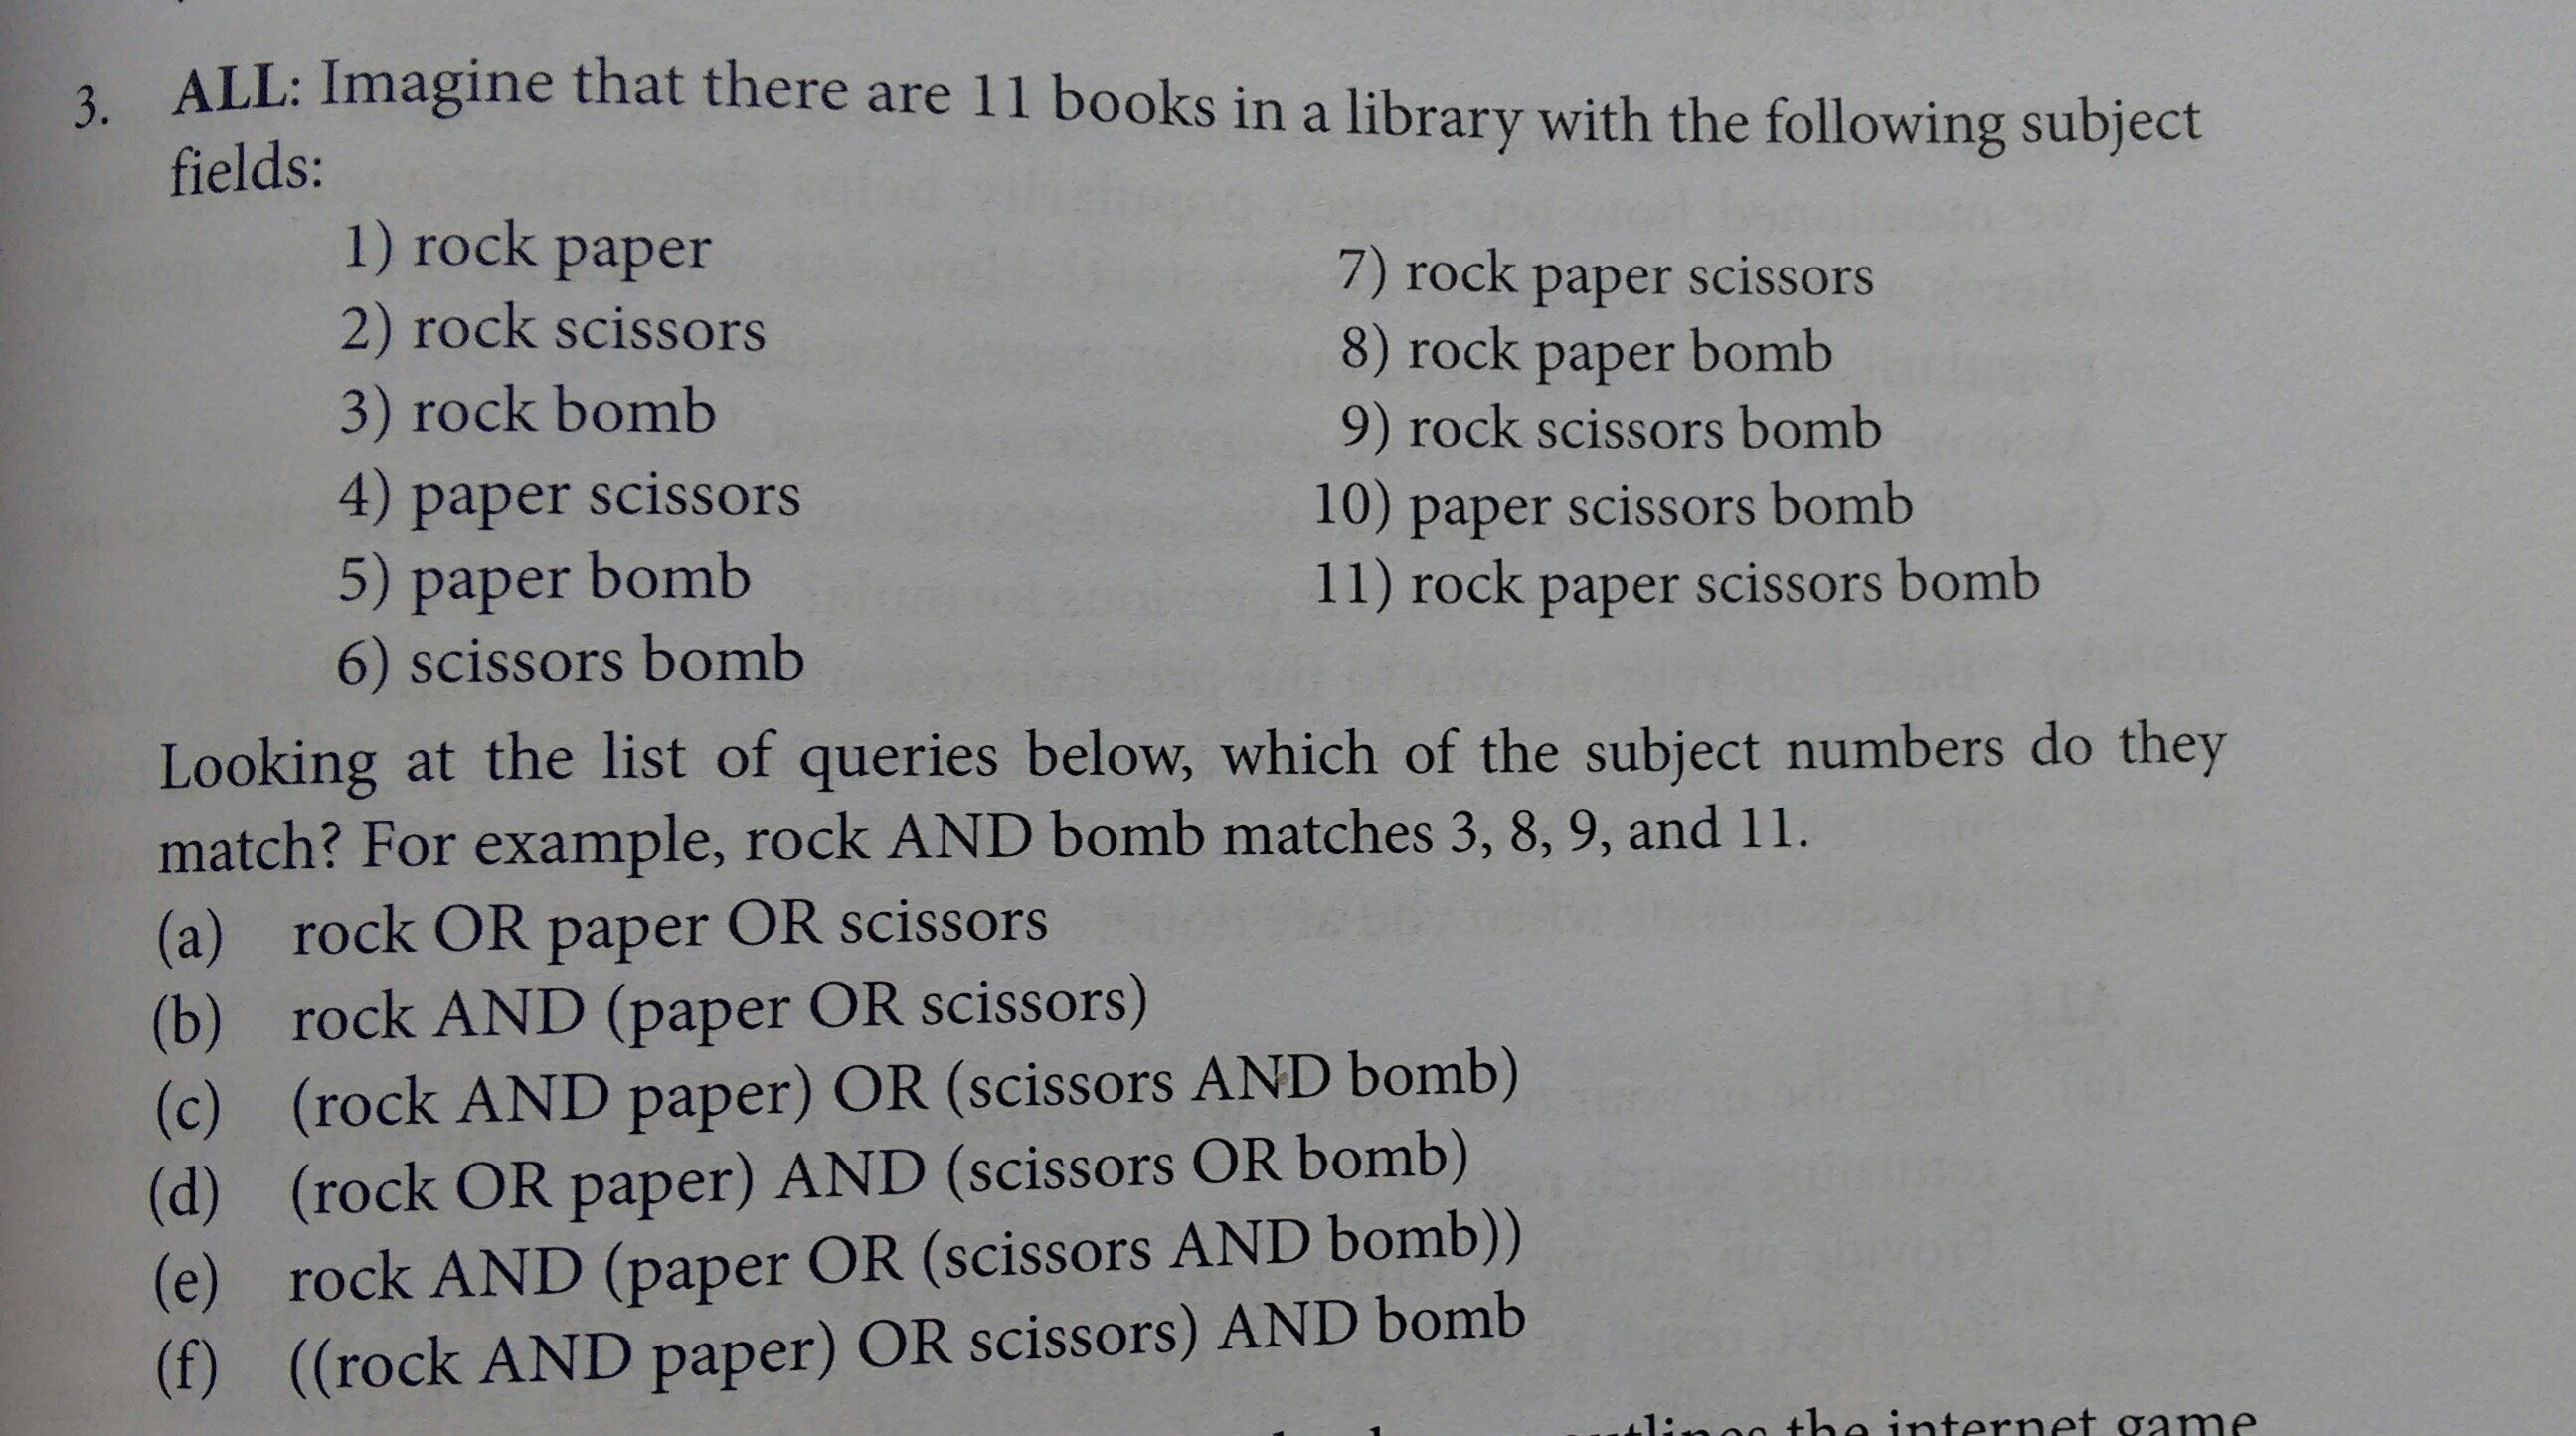
\includegraphics[width=0.9\textwidth]{Q1.jpg}
\end{frame}

\begin{frame}
\frametitle{Questions to resolve by Friday}
\begin{itemize}
\item Okay, indexing is cool. But for any query, I may still end up with 10000 results. How can I rank them?
\item How do I ensure only good quality pages get ranked on top. 
\end{itemize}
\end{frame}

\begin{frame}
\frametitle{Attendance Exercise(s) - Lots of questions}
Think about these problems and submit your thoughts online on Canvas forum for today. 
\begin{itemize}
\item Is "popularity" a good heuristic to rank a page? Provide one example where your search query results in a popular page as the top result, but is incorrect for your need. What is the rank of the page that met your need?
\item Question on Googlewhack. That website in the picture does not work though. You should use other means to know more.  
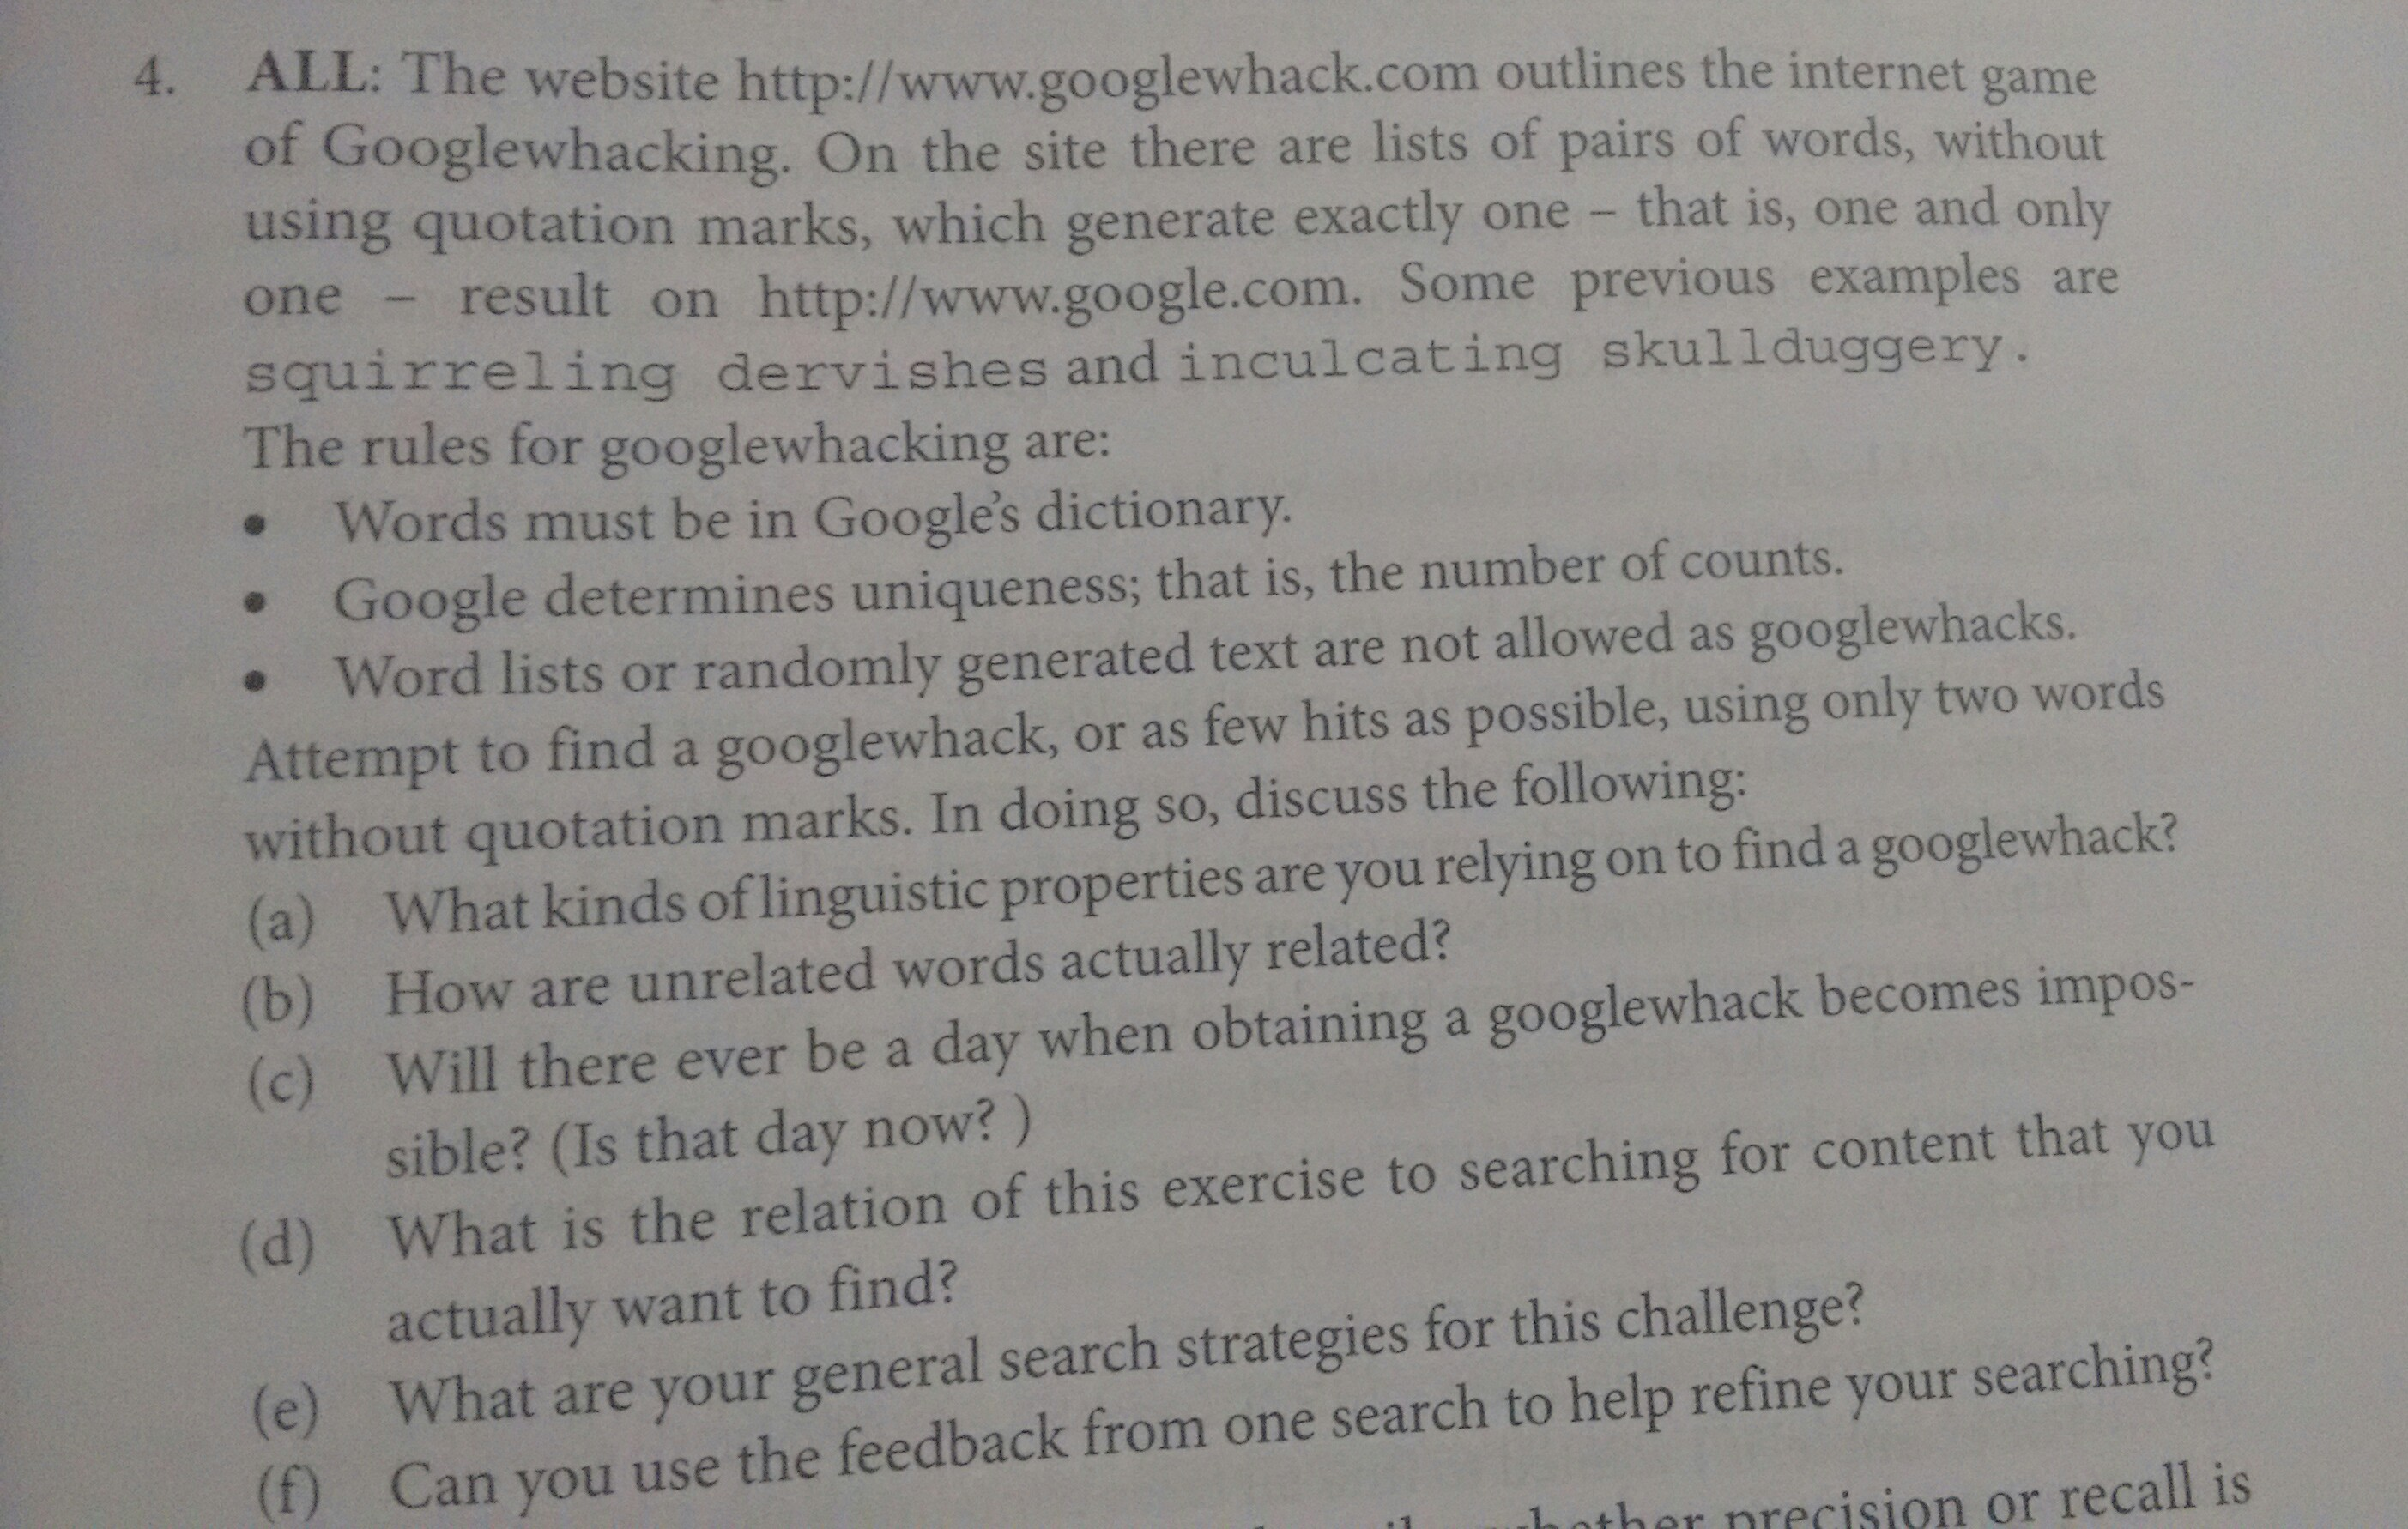
\includegraphics[width=0.6\textwidth]{20Sep-120Exercise.jpg}
\end{itemize}
\end{frame}%Majuvanchara gave only one result.

\end{document}
